\chapter{Results}
As all the necessary requirements for the PEEPS framework presented in 3.1.2 were fulfilled, testing on the both the application and server systems could commence. The experimental setup and findings for this project are details in this section.


\section{Final Product Presentation}
The final product was tested on a OnePlus 7 Pro smartphone with its GPS and network location services enabled. The device contains a Snapdragon 855 processor, a 1440p display and 6GB of RAM.

\begin{figure}
    \centering
    \begin{minipage}{.5\textwidth}
      \centering
      \frame{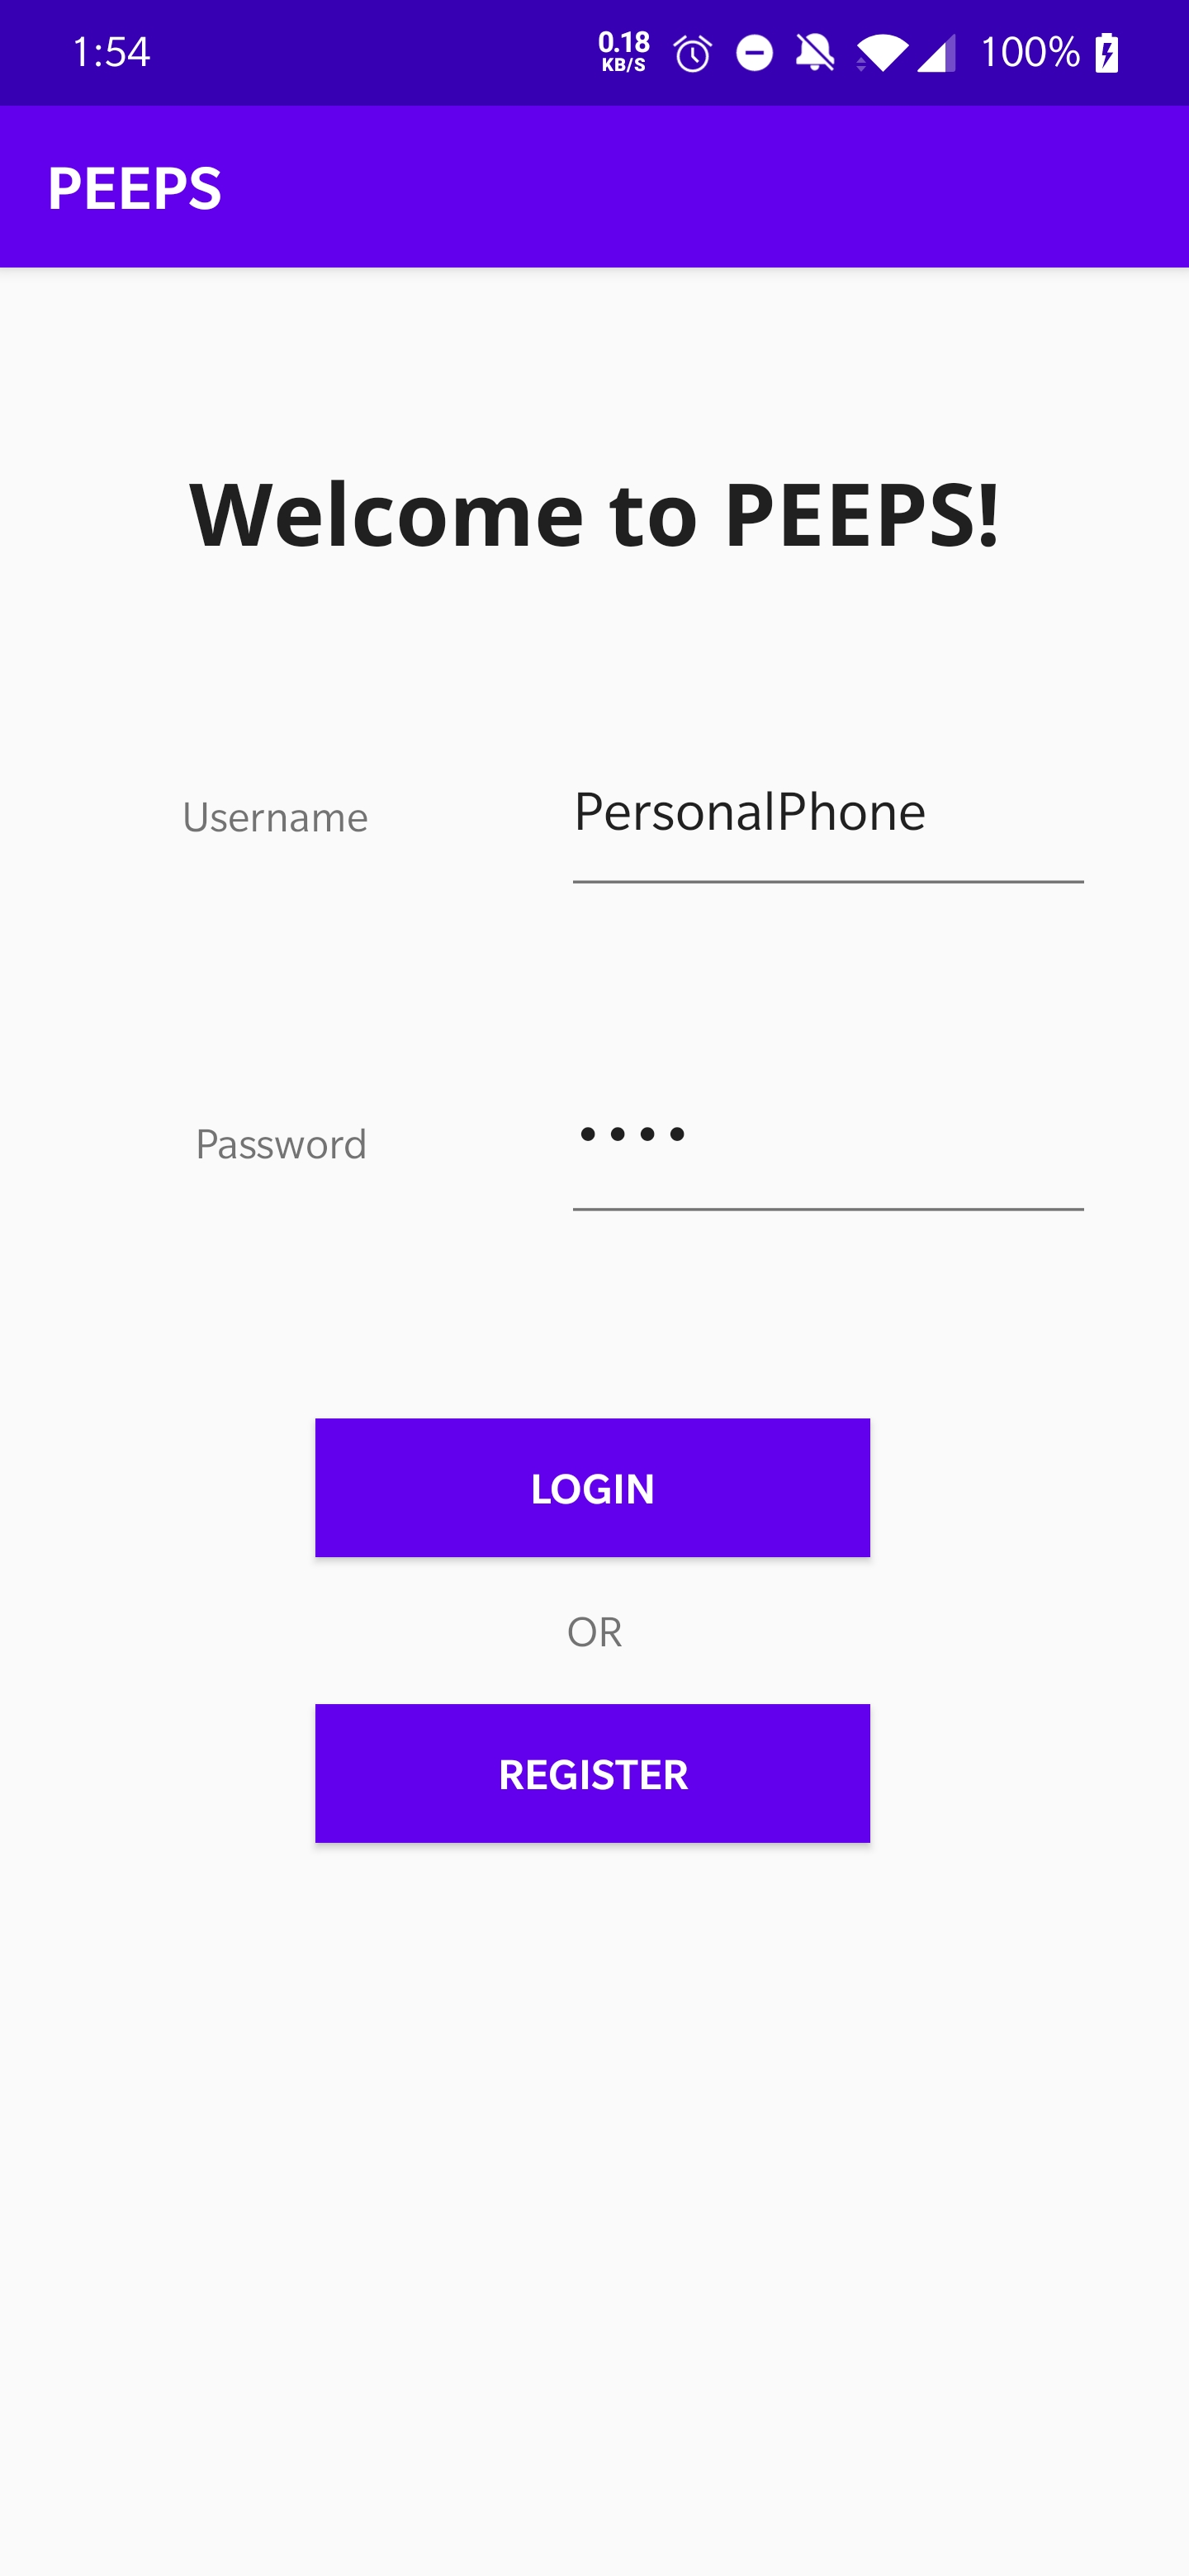
\includegraphics[width=.6\linewidth]{figures/ResultLogin.jpg}}
      \caption{Login-and-welcome view.}
      \label{fig:results_login}
    \end{minipage}%
    \begin{minipage}{.5\textwidth}
      \centering
      \frame{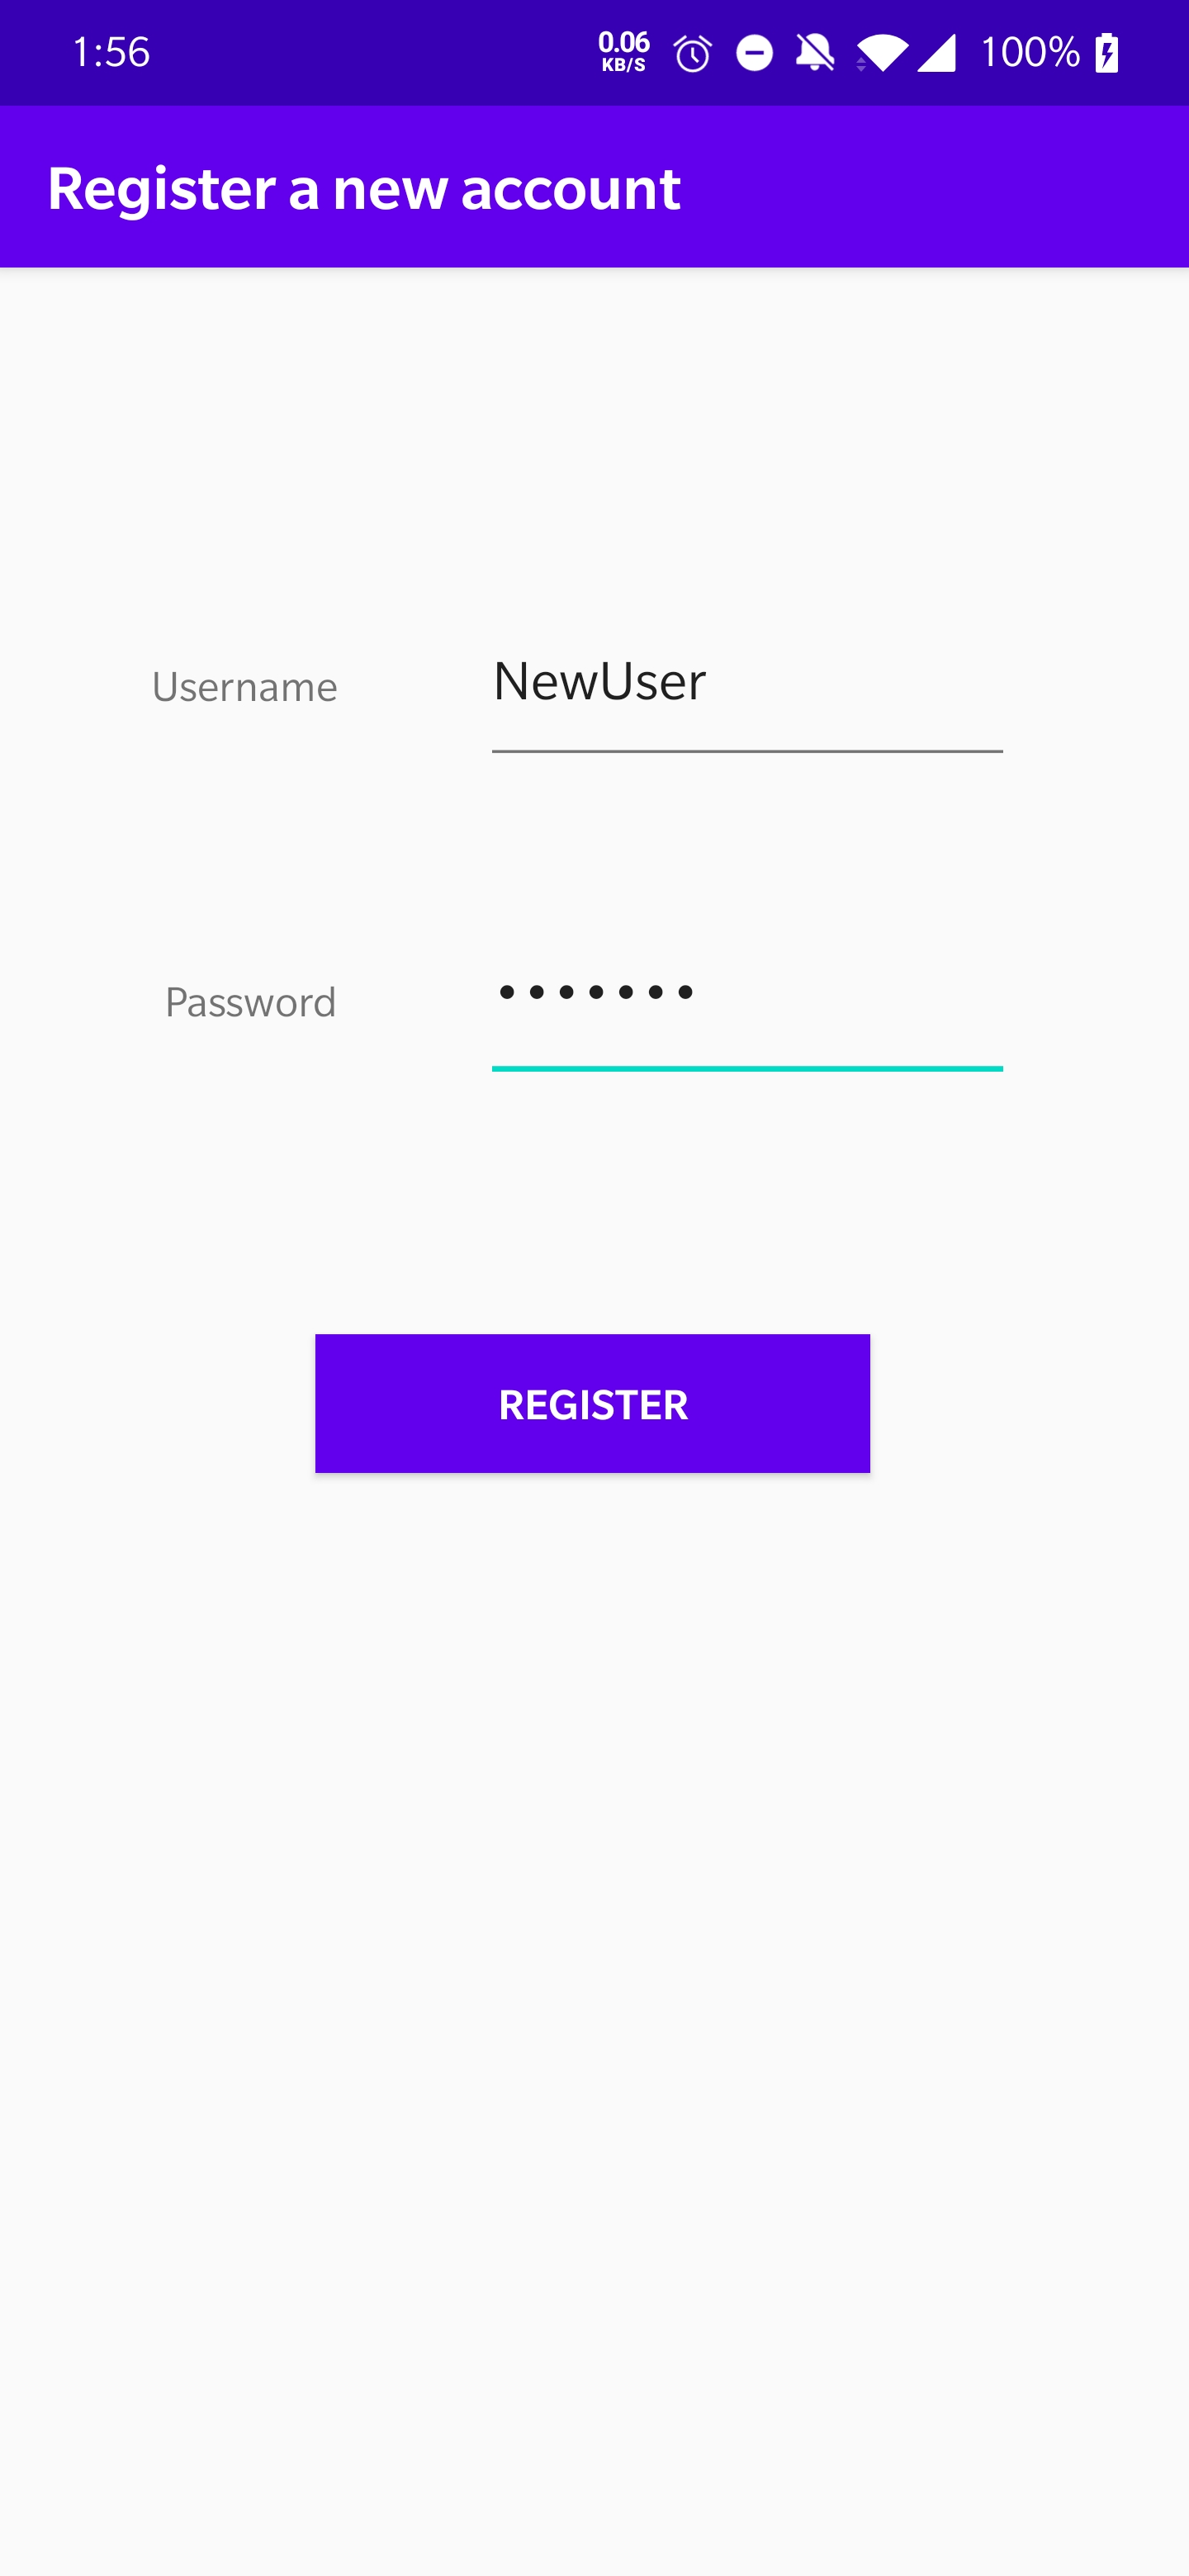
\includegraphics[width=.6\linewidth]{figures/ResultRegister.jpg}}
      \caption{Register-user view.}
      \label{fig:result_register}
    \end{minipage}
\end{figure}

The login and register GUIs are built with simplicity and usability as its core design principles. The input fields are centred and take up most of the screen’s interactive space, while the actions that the user can take are displayed as highly contrasted buttons. These views also highlight the theme that was decided for this app which is a clean light grey background with purple interactable elements. 

\begin{figure}
    \centering
    \begin{minipage}{.5\textwidth}
      \centering
      \frame{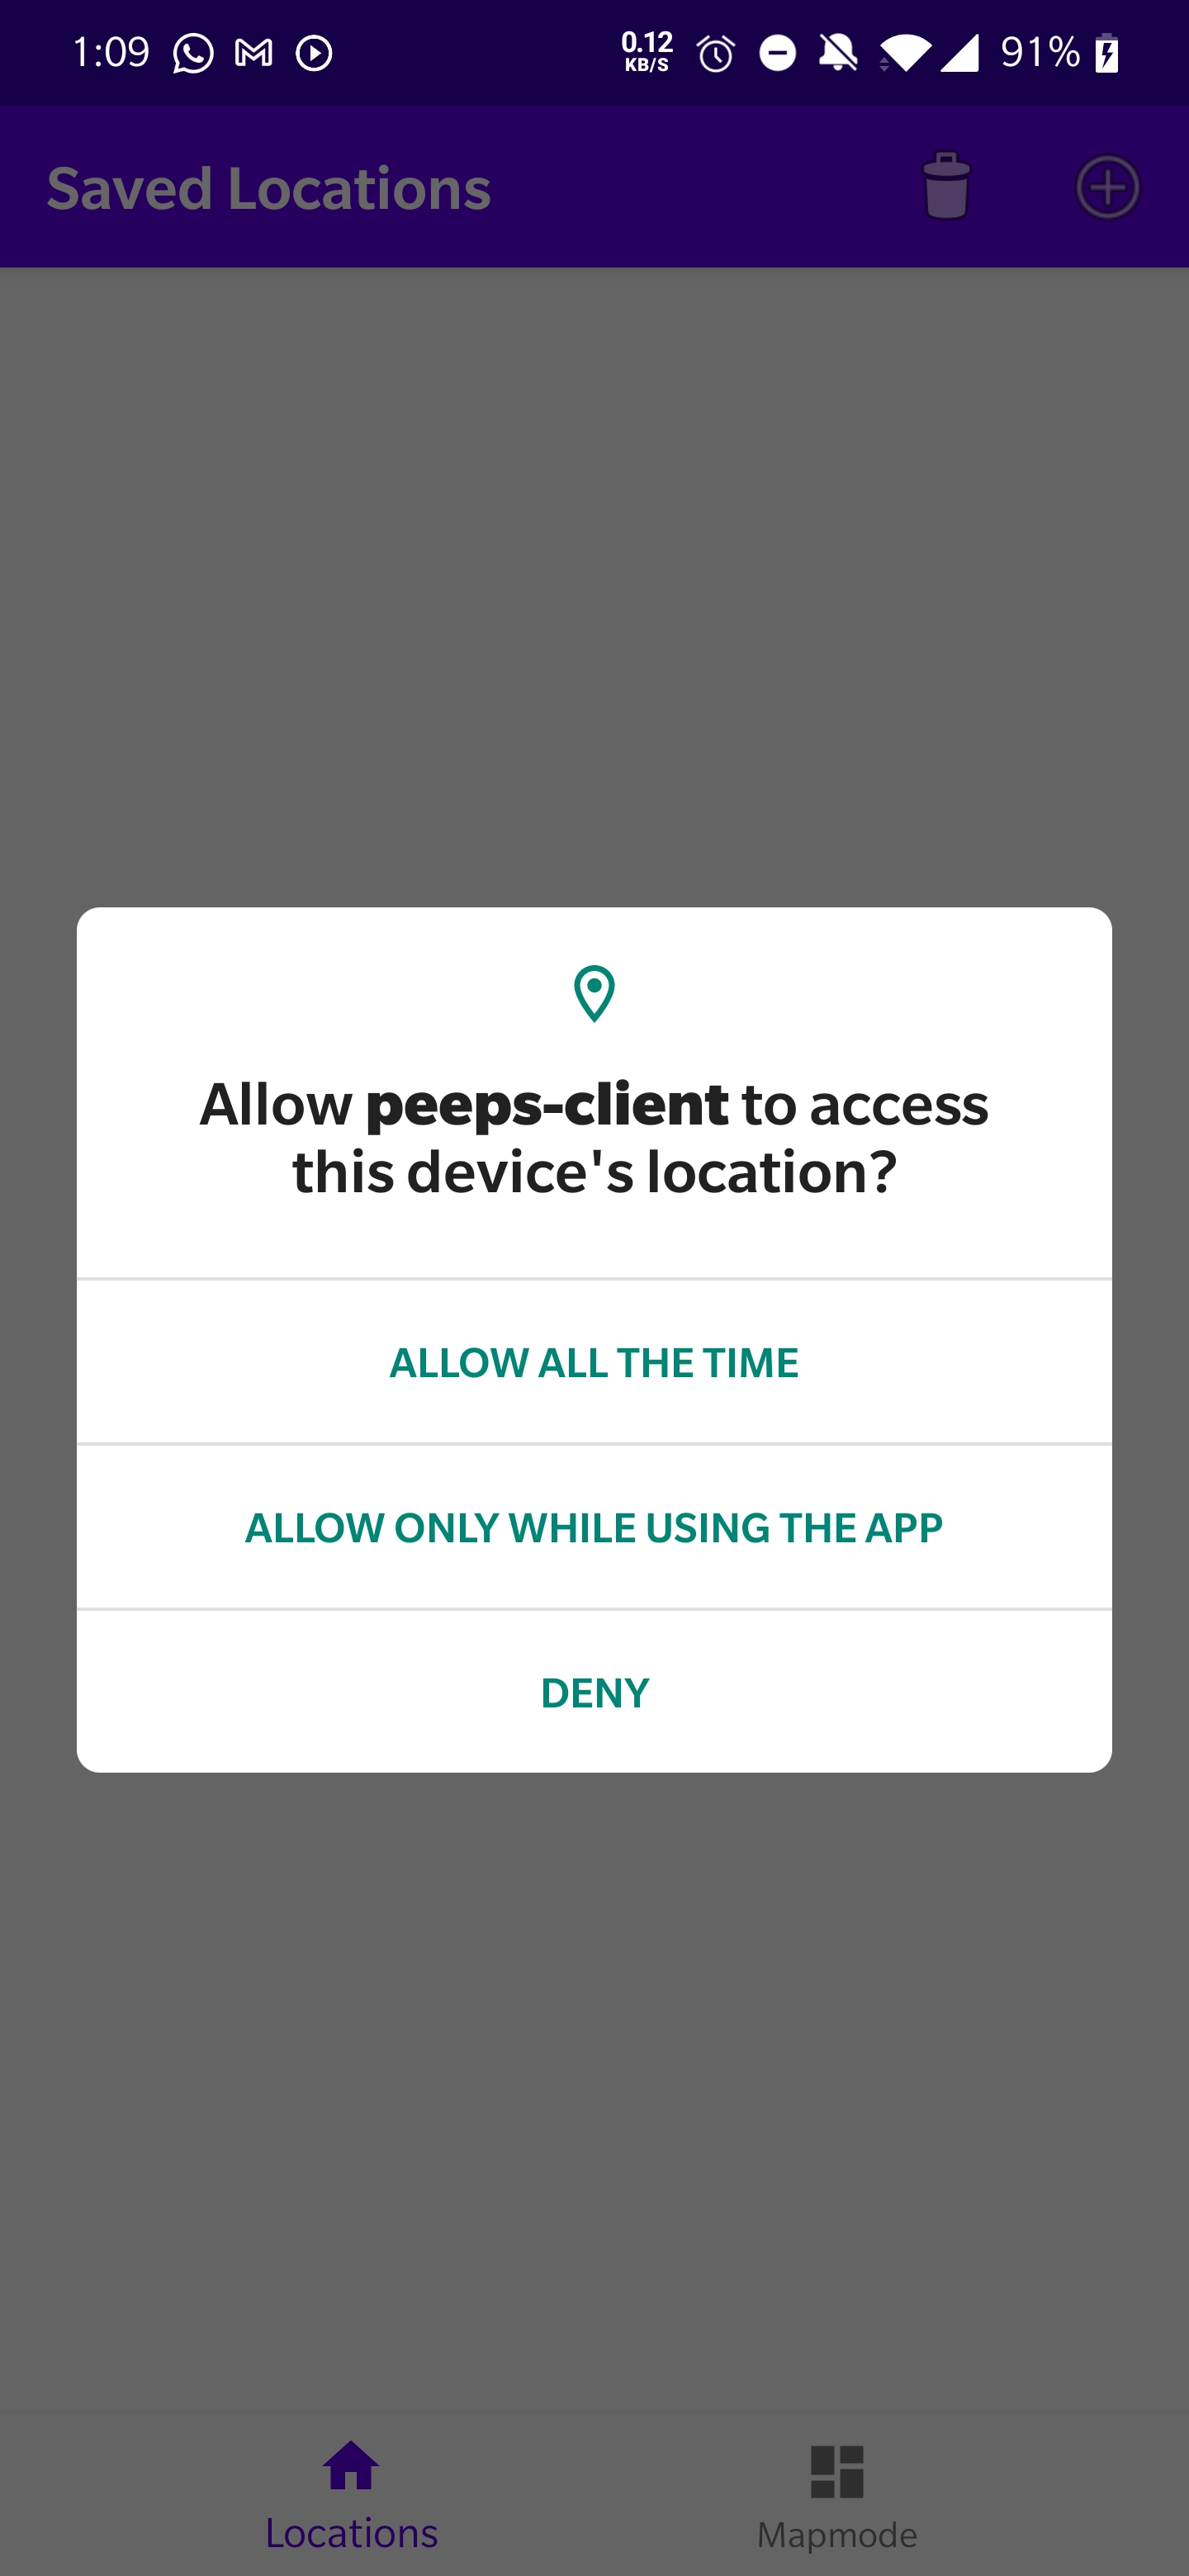
\includegraphics[width=.6\linewidth]{figures/ResultPermission.jpg}}
      \caption{Location permission alert shown when user logs in.}
      \label{fig:result_permission}
    \end{minipage}%
    \begin{minipage}{.5\textwidth}
        When the user first logs into the app after making an account, they will be asked to allow the app to access their location. Without this feature, the user will not be able to contribute their location to the crowd sourcing database. The app will however still function without this feature enabled.
    \end{minipage}
\end{figure}

\begin{figure}
    \centering
    \begin{minipage}{.5\textwidth}
      \centering
      \frame{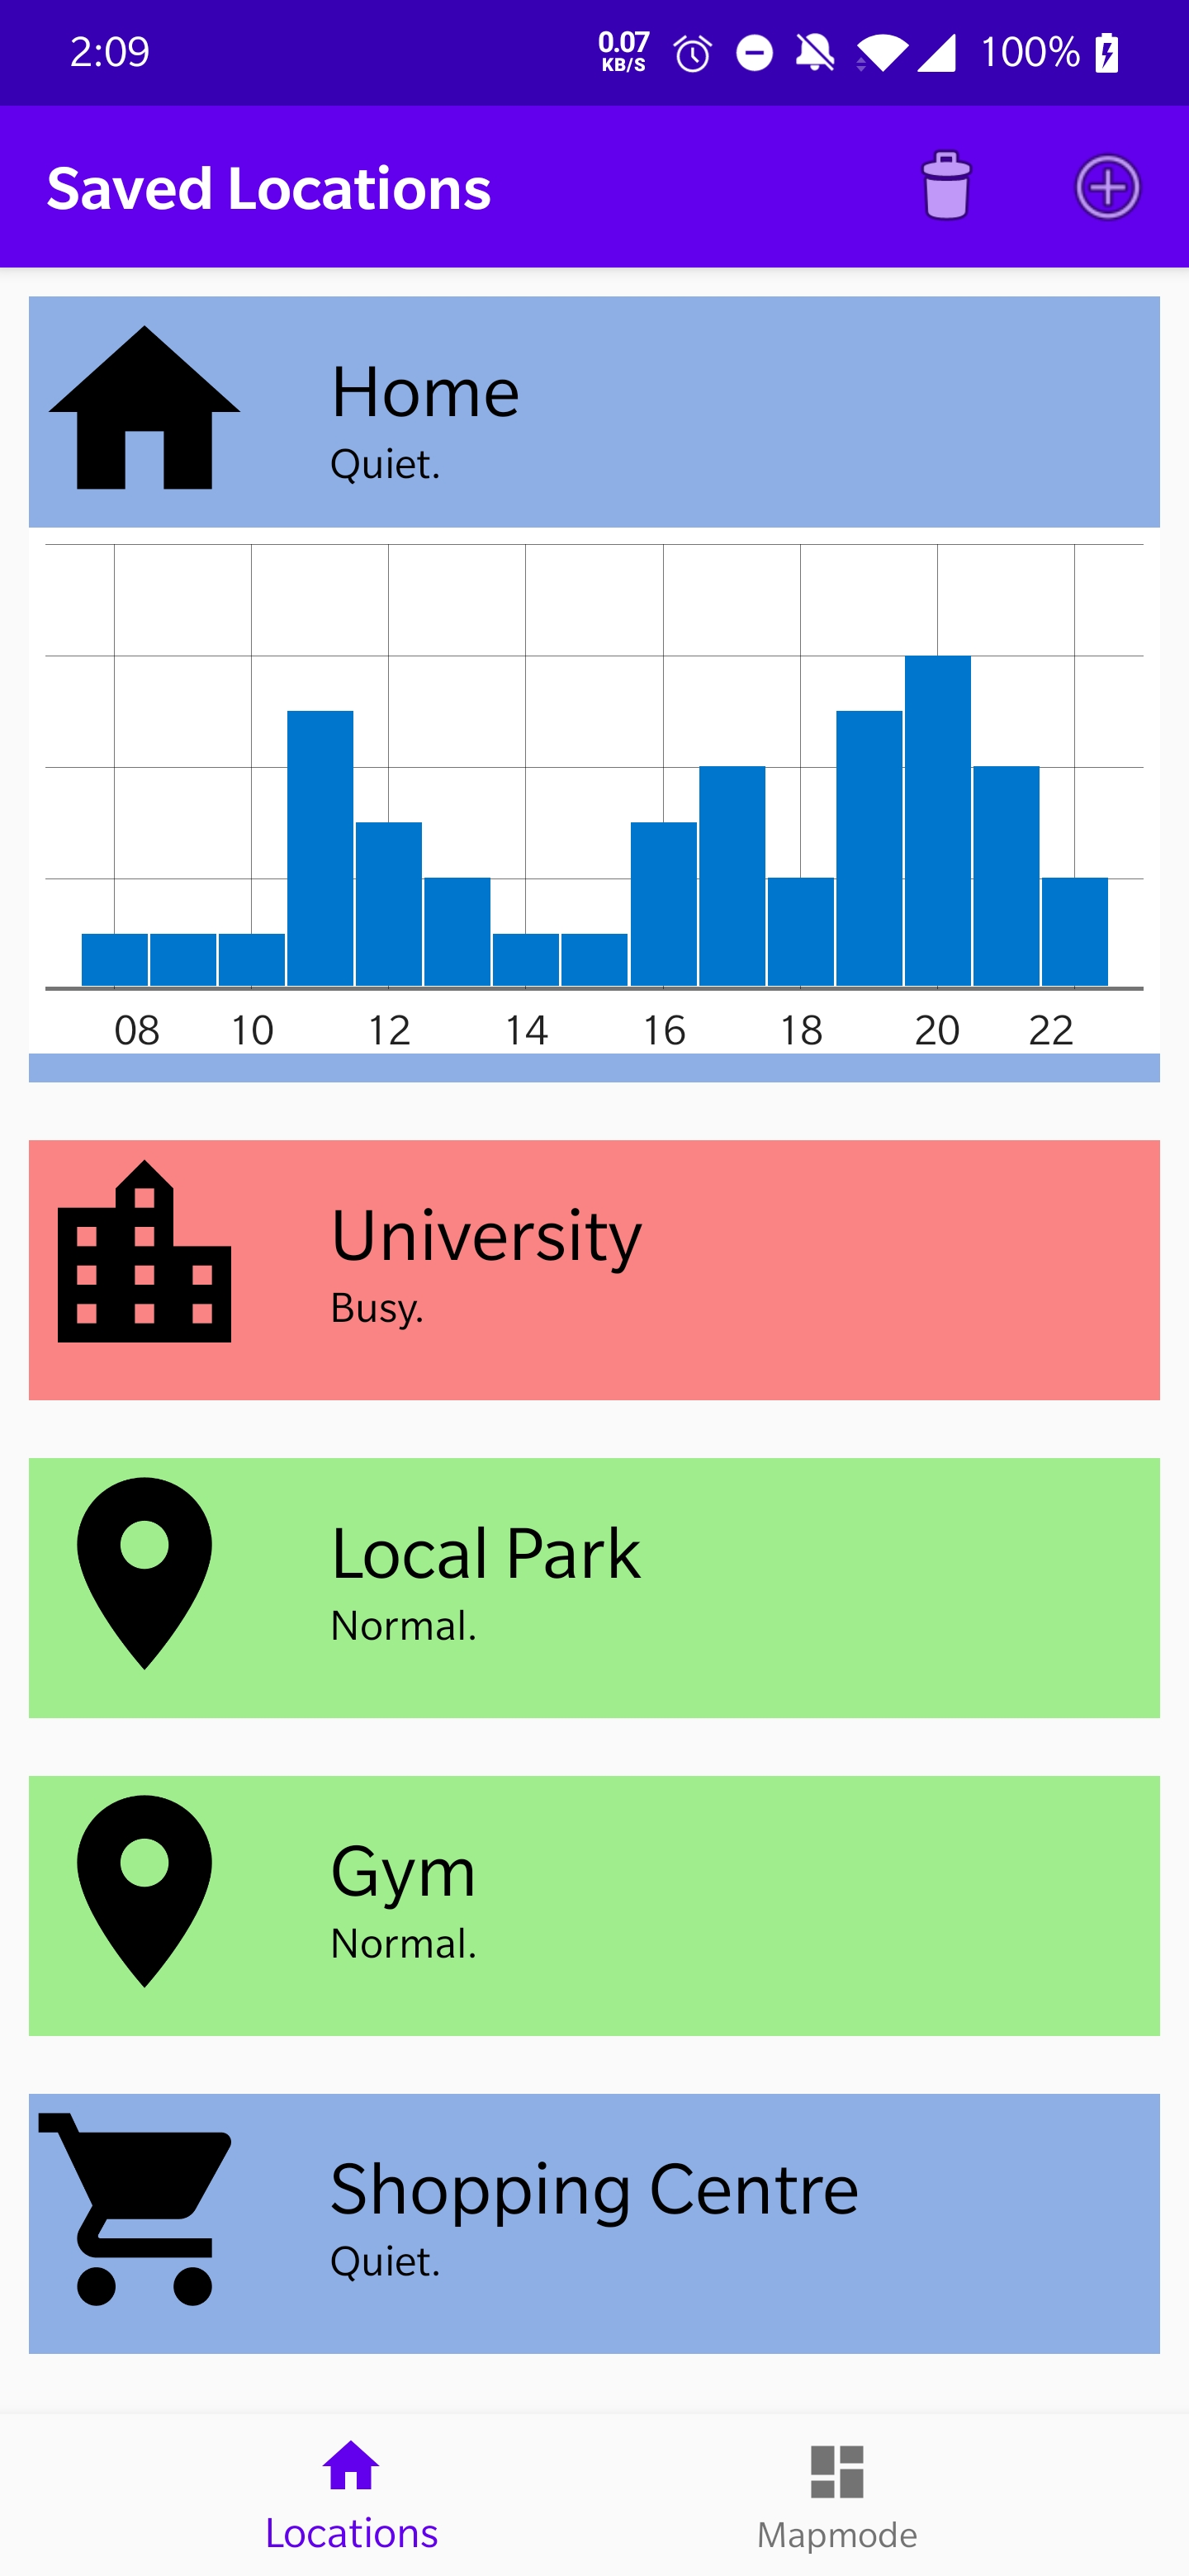
\includegraphics[width=.6\linewidth]{figures/ResultExtended.jpg}}
      \caption{Extended saved-location view.}
      \label{fig:result_extended}
    \end{minipage}%
    \begin{minipage}{.5\textwidth}
      \centering
      \frame{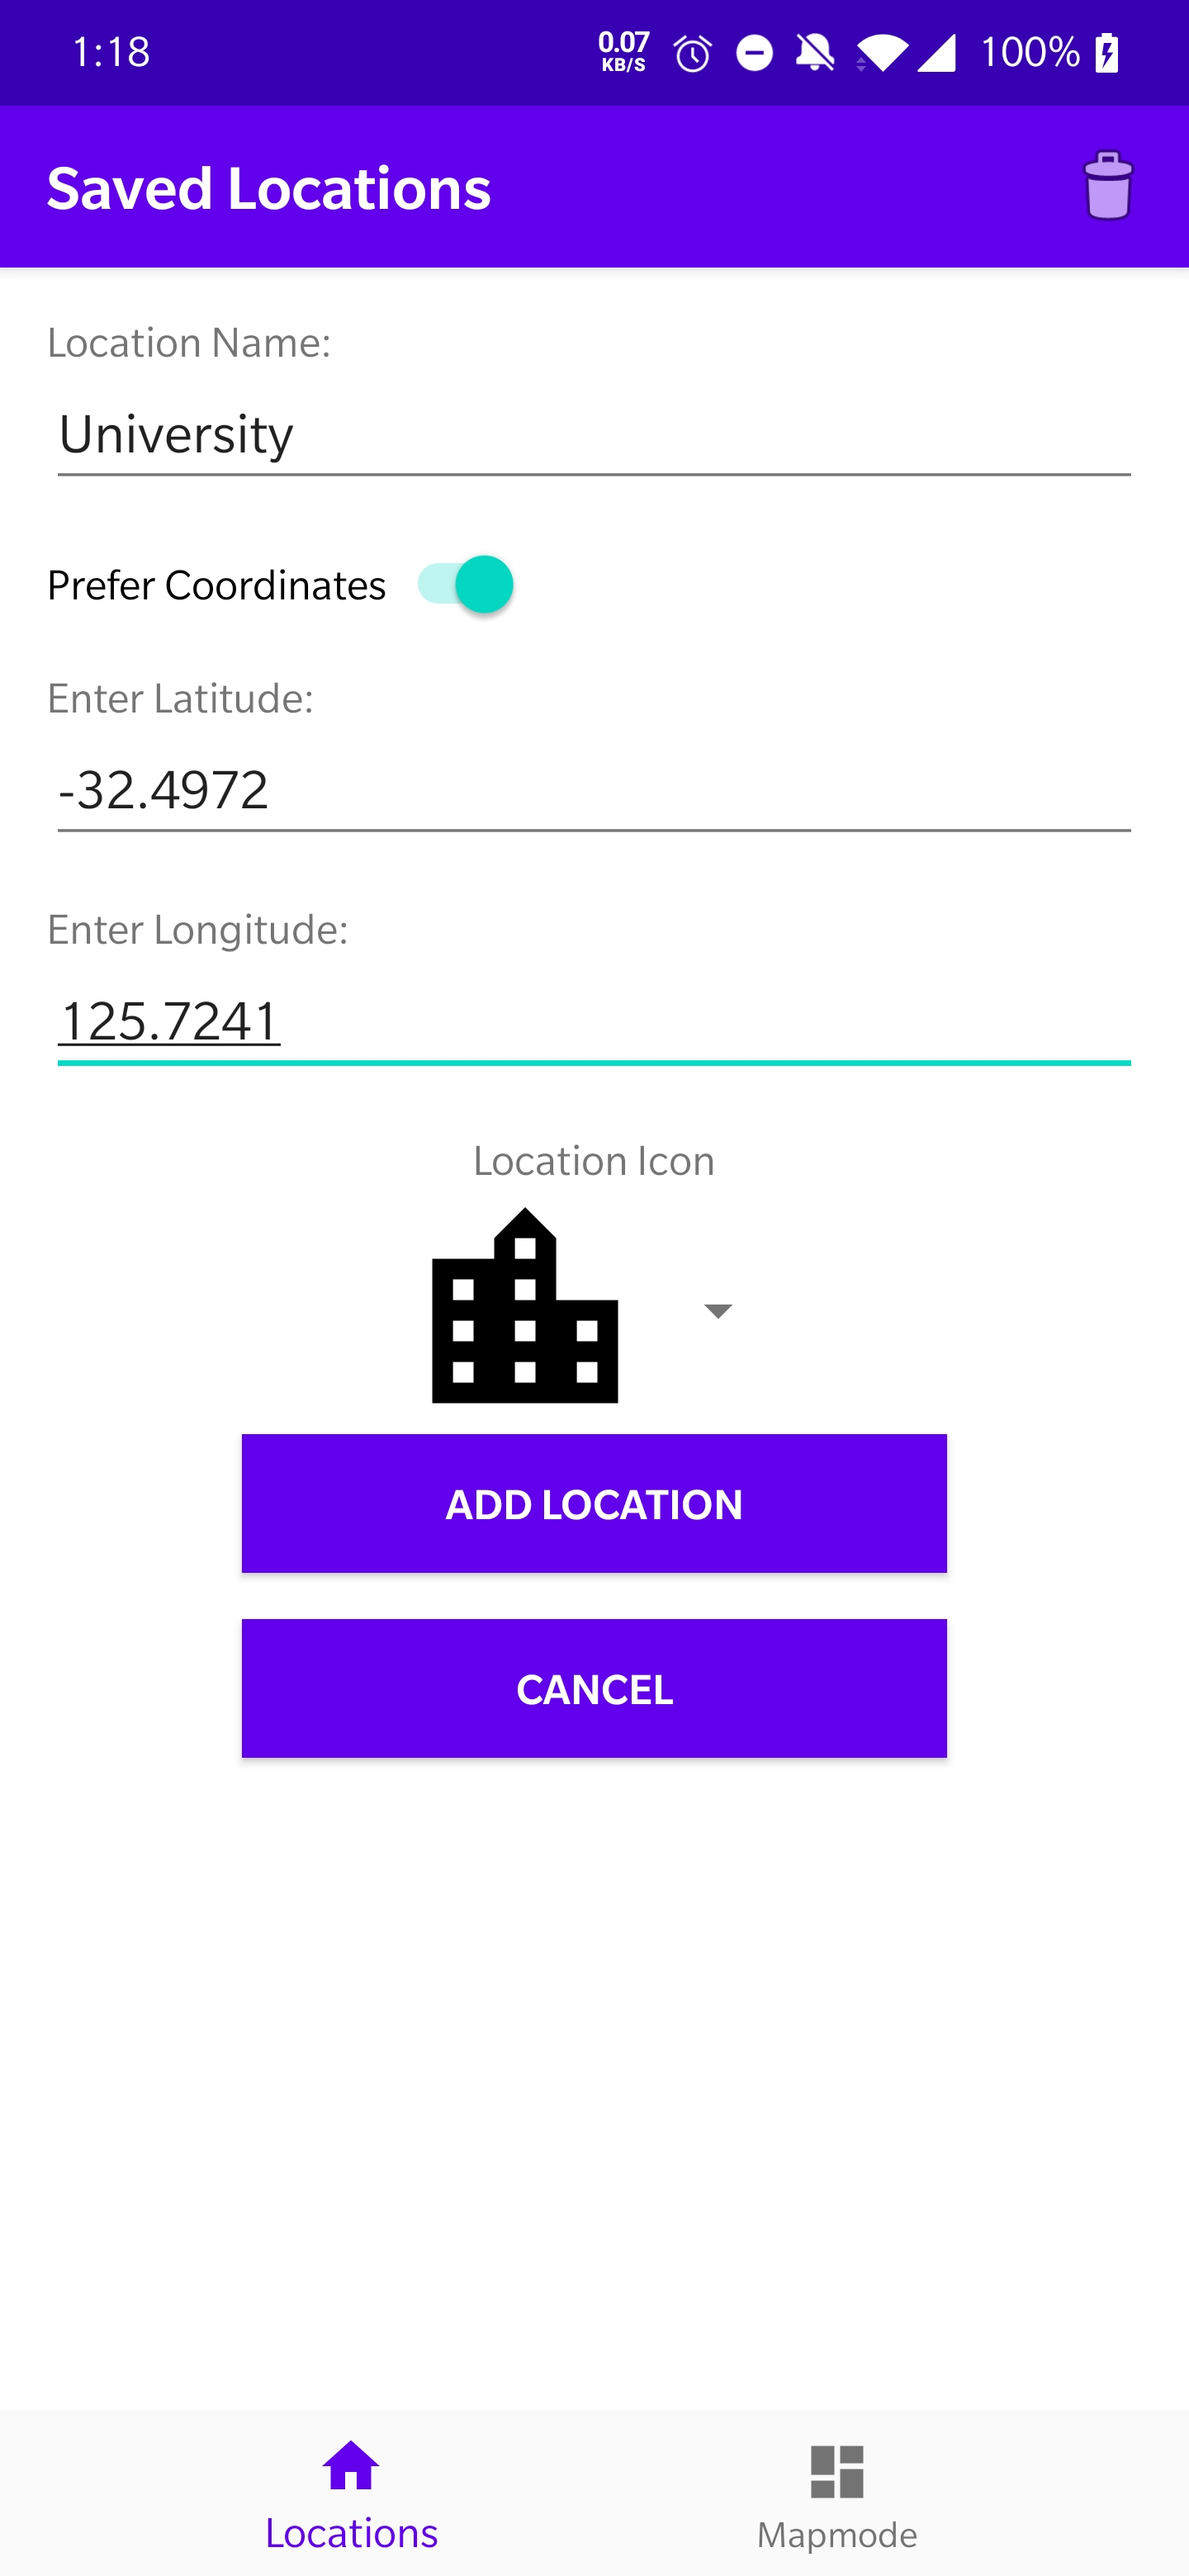
\includegraphics[width=.6\linewidth]{figures/ResultAdd.jpg}}
      \caption{New-saved-location view with 'prefer coordinates' selected.}
      \label{fig:result_add}
    \end{minipage}
\end{figure}

The views in Figure \ref{fig:result_extended} and Figure \ref{fig:result_add} show the main functionality of the application. Figure X is the main page of the app displaying the user’s saved locations and their current population status. For the purpose of testing these locations’ population data was artificially inserted into the database to provide insight into ow the app would look under actual usage conditions. Figure \ref{fig:result_add} displays the Dialog Fragment which overlays the view of figure \ref{fig:result_extended}. Here the user inputs the name, icon, and coordinates of a new location.

The GUI from the mapmode fragment is shown in the results page in Figure TODO.

\subsection{Application Interaction Feedback Mechanisms}
It is important when designing a user interface that the user is presented with dynamic methods of interaction to help inform them of the results of their actions. The PEEPS application implements this by displaying ‘toasts’. These are temporary update messages which inform the user of a background process that they would benefit from knowing is happening. 

\begin{figure}[ht]
    \centering
    \frame{
\includegraphics[width=0.7\textwidth]{figures/ResultToast.jpg}}
    \caption{Successful login toast}
    \label{fig:result_toast}
\end{figure}

Another way the application provides feedback to the user is the transition between an item of figure \ref{fig:result_extended} being expanded and closed. When the item is selected the location card will slowly expand and the graph will become visible. This transition makes the user interaction less sudden and ensures they understand the consequences of selecting an item in the list.

\section{Functional Testing}
TEST-1: \textbf{Location Status Test}

For this first test, a list of user locations was manually added to the database with a constant set of coordinates. The amount of locations added to the database were equal to three times the time bracket at which their location was hypothetically taken, with a timestamp dating a week earlier than the test day. Because the web interface averages data from the previous three weeks before the request, we expect to see a linearly increasing graph on the app when analysing data from the correct coordinates.
When the same coordinates were added as a saved location to the app, the resulting graph displayed a linearly increasing population. This verifies the app’s ability to use the Saved Location View to display accurate information about the status of chosen locations.

TEST-2: \textbf{Best Route Test}

A list of user’s data was manually inserted into the database for four different locations. The app’s Mapmode fragment was activated to calculate the best time to leave on a journey through each of these locations to minimise the amount of people who the user would be in close proximity to. The ideal departure time and amount of contact with people was output to the device. The data added can be viewed in appendix TODO.

\begin{figure}[ht]
    \centering
    \frame{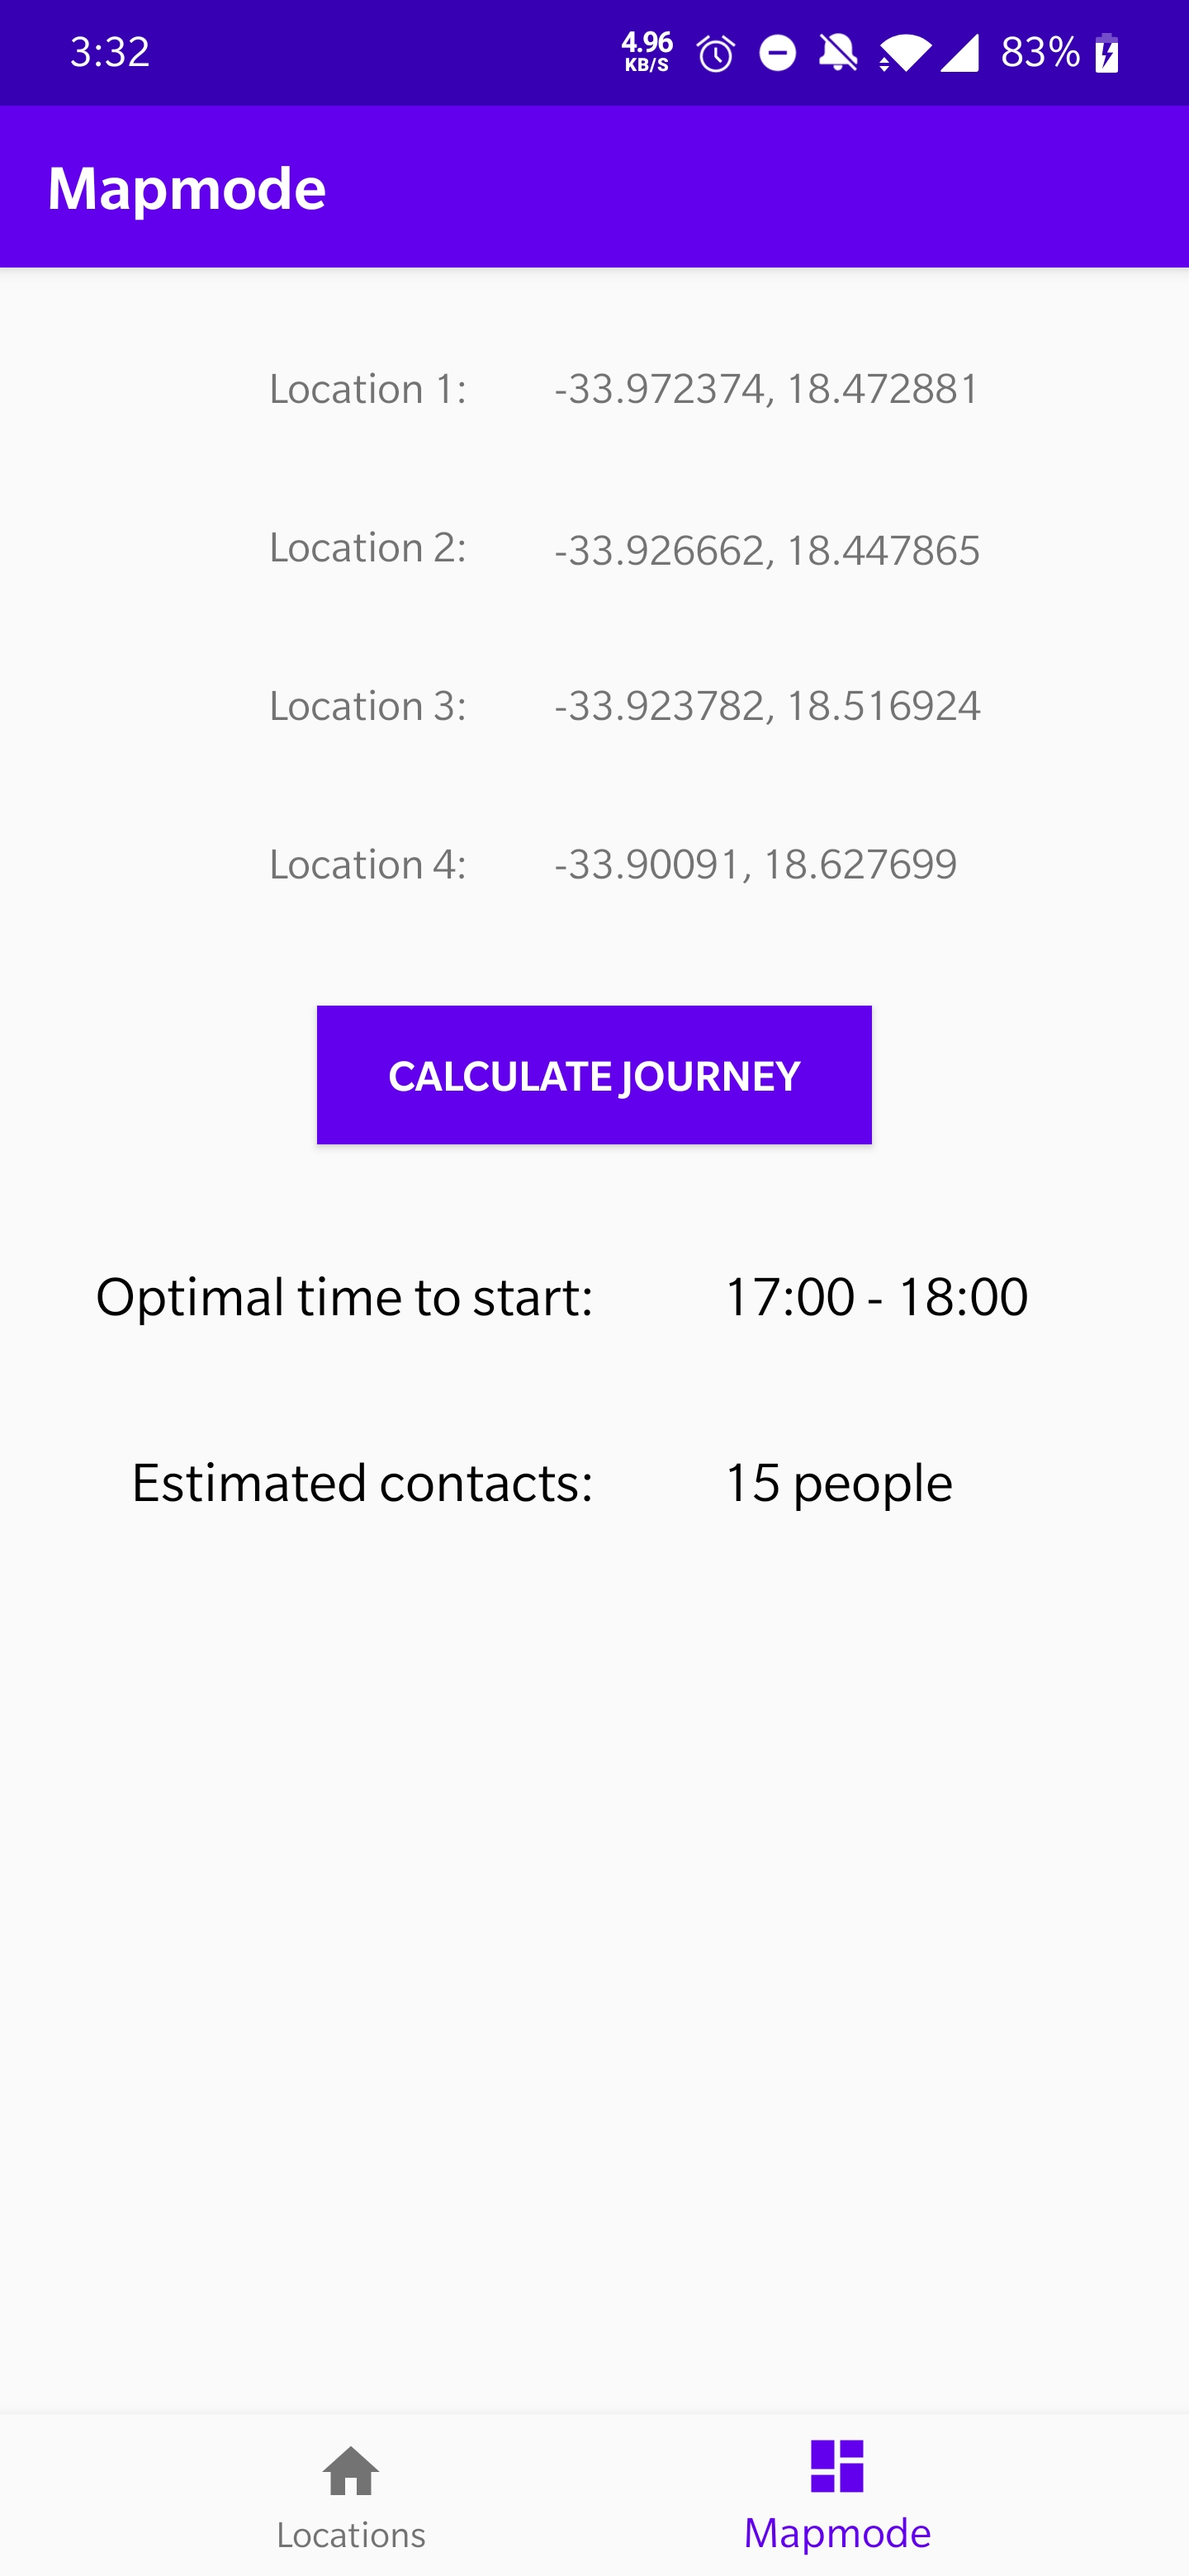
\includegraphics[width=0.7\textwidth]{figures/ResultMapmode.jpg}}
    \caption{Mapmode displaying the optimal start-time and estimated contacts.}
    \label{fig:result_mapmode}
\end{figure}

The control, performed in excel, verifies that the app is able to determine the optimal time to begin the route when minimising person-to-person contact. The control can be viewd in apendix TODO.

\subsubsection{Functional Analysis}

The Location Status and Best Route tests both show that the app can function correctly while providing the user with important population information. This information can be used to make meaningful decisions like when to visit a generally crowded area, how populated a business owners’ shops are and when best to go out on your planned trip to minimise chance of infection. The success of the tests indicate that the app meets its functional requirement of providing a useful service to the user.

\section{Investigative Testing}

TEST-3: \textbf{Location Accuracy Test}

For this test, a smartphone with the app installed was left in a stationary location for four hours so that it had sufficient time to make location updates. The normal frequency at which the location was uploaded was also artificially increased for the purpose of this test. The scatter of coordinates that were uploaded to the database were recorded and analysed. Because the distribution of the locations is assumed to be gaussian, the uncertainty was calculated using a Type A evaluation. This method uses a combination of the mean and standard deviation to determine the bounds of how accurate the location is. Note that because the smartphone’s location is determined by the phone’s GPS and network sensor, the accuracy of location gathering will differ from phone to phone.

To determine the uncertainty of the phones location gathering capabilities, first the coordinate system was zeroed on the mean and each coordinate was converted from degrees into the distance from the mean in meters. This was used to calculate the standard deviation and uncertainty as follows:



\section{Verification of Specifications}



\section{Discussion}